\documentclass{beamer}
%Information
\title{Geometry 2: Circle}
\titlegraphic{\hfill
\includegraphics[height=1cm]{orange.png}}
\institute{Youth STEM Academy}
\author{Erzhuo Wang}
\date{July 10,2024}
%Theme
\usetheme[block=fill, sectionpage=none]{metropolis}
\useoutertheme{infolines}
\useinnertheme{metropolis}
\setbeamertemplate{blocks}[rounded][shadow=false]
\setbeamertemplate{items}[ball]
\setbeamertemplate{sections/subsections in toc}[ball]
\setbeamertemplate{headline}{}
\logo{YSA}
\usecolortheme{custom}

%Setting
\usepackage[UTF8,noindent]{ctexcap}
\theoremstyle{definition}
\newtheorem{defn}{Definition}[section]
\newtheorem{coro}[defn]{Corollary}
\newtheorem{theo}[defn]{Theorem}
\newtheorem{exer}[defn]{Exercise}
\newtheorem{rema}[defn]{Remark}
\newtheorem{lem}[defn]{Lemma}
\newtheorem{prop}[defn]{Proposition}
\newtheorem{nota}[defn]{Notation}
\newtheorem{exam}[defn]{Example}
\newtheorem{ques}[defn]{Question}

\newenvironment{prooff}{{\noindent\it\textcolor{cyan!40!black}{Proof}:}\,}{\par}
\newenvironment{proofff}{{\noindent\it\textcolor{cyan!40!black}{Proof of the lemma}:}\,}{\qed \par}
\newcommand{\bbrace}[1]{\left\{ #1 \right\} }
\newcommand{\bb}[1]{\mathbb{#1}}
\newcommand{\p}{^{\prime}}
\renewcommand{\mod}[1]{(\text{mod}\,#1)}
\newcommand{\blue}[1]{\textcolor{blue}{#1}}
\newcommand{\spec}[1]{\text{Spec}({#1})}
\newcommand{\rarr}[1]{\xrightarrow{#1}}
\newcommand{\larr}[1]{\xleftarrow{#1}}
\newcommand{\emptyy}{\underline{\quad}}
\newenvironment{enu}{\begin{enumerate}[(1)]}{\end{enumerate}}
%ctrl+点击文本返回代码  选中代码 ctrl+alt+j 为代码查找文本
\begin{document}
\begin{frame}
    \titlepage
\end{frame}
\begin{frame}{Semi-Circle 1}
    \begin{ques}
        In the right triangle $A B C, A C=12, B C=5$, and angle $C$ is a right angle. A semicircle is inscribed in the triangle as shown. What is the radius of the semicircle?

        在直角三角形$ABC$中, $A C=12$, $BC=5$, 角$C$是一个直角.如图所示,三角形内嵌了一个半圆, 求半圆的半径.
    \end{ques}
    \begin{figure}
        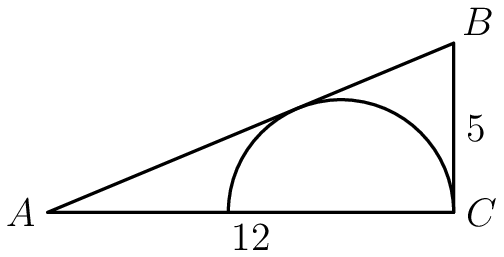
\includegraphics[height=0.4\textheight]{triangle4.png}
    \end{figure}
\end{frame}
\begin{frame}{Semi-Circle 2}
    \begin{ques}
        A semicircle is inscribed in an isosceles triangle with base $16$ and height $15$ so that the diameter of the semicircle is contained in the base of the triangle as shown. What is the radius of the semicircle?

        一个半圆内嵌在一个底16高15的等腰三角形中,这样半圆的直径就包含在三角形的底中,求半圆半径.
    \end{ques}
    \begin{figure}
        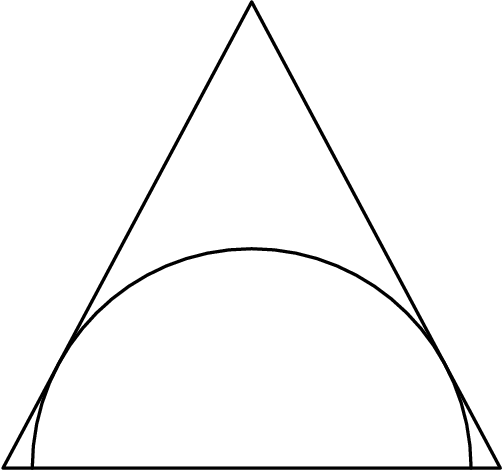
\includegraphics[height=0.4\textheight]{circle1.png}
    \end{figure}
\end{frame}
\begin{frame}{Circle-1}
    \begin{ques}[AMC 8, 2014-15]
        The circumference of the circle with center $O$ is divided into 12 equal arcs, marked the letters $A$ through $L$ as seen below. What is the number of degrees in the sum of the angles $x$ and $y$?

        将圆等分为$12$份, 求$x$和$y$的角度之和.
    \end{ques}
    \begin{figure}
        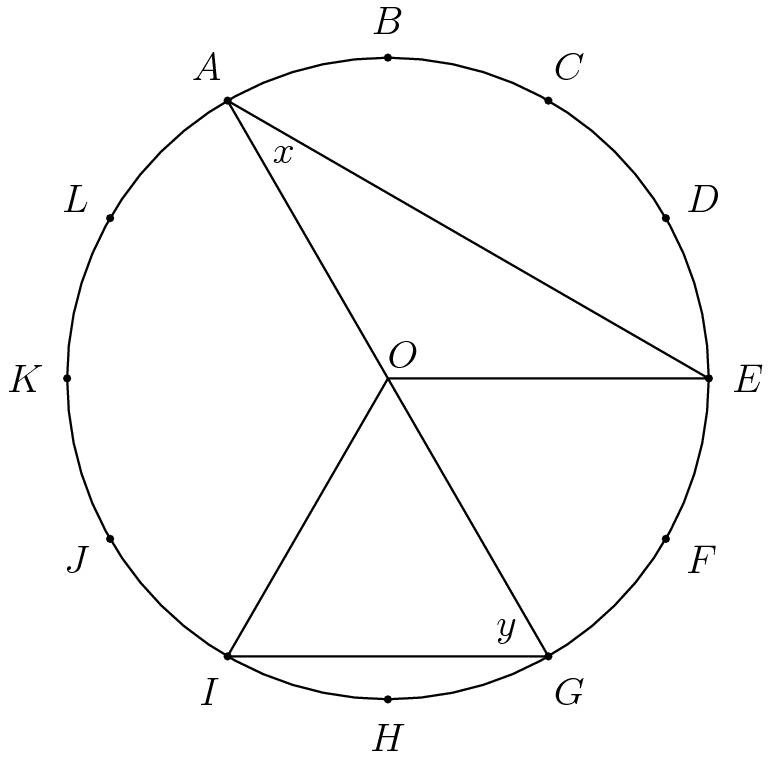
\includegraphics[height=0.4\textheight]{circle2.png}
    \end{figure}
\end{frame}
\begin{frame}{Circle-2}
    \begin{ques}[AMC 8, 2014-20]
        $CD=3$, $DA=5$. 圆心为$A$的圆半径为$1$, 圆心为$B$的圆半径为$2$, 圆心为$C$的圆半径为$3$, 求被三个圆割剩下的矩形面积.
    \end{ques}
    \begin{figure}
        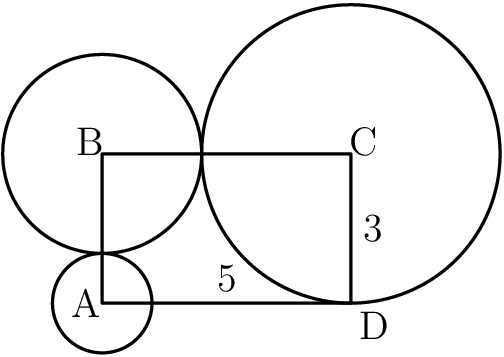
\includegraphics[height=0.4\textheight]{circle3.png}
    \end{figure}
\end{frame}
\begin{frame}{Circle-3}
    \begin{ques}[AMC 8, 2013-23]
        Angle $ABC$ of $\triangle ABC$ is a right angle. The sides of $\triangle ABC$ are the diameters of semicircles as shown. The area of the semicircle on $\overline{AB}$ equals $8\pi$, and the arc of the semicircle on $\overline{AC}$ has length $8.5\pi$. What is the radius of the semicircle on $\overline{BC}$?

        以$AB$为直径的半圆面积为$8\pi$, 圆弧$AC$长为$8.5\pi$, 求$BC$的长度.
    \end{ques}
    \begin{figure}
        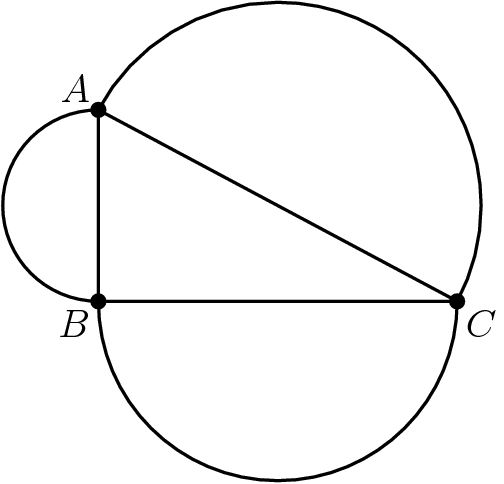
\includegraphics[height=0.4\textheight]{circle4.png}
    \end{figure}
\end{frame}

\begin{frame}{Circle-4}
    \begin{ques}[AMC 8, 2010-19]
        如图, $AC=10$, $AD=16$, 求两圆中间圆环的面积.
    \end{ques}
    \begin{figure}
        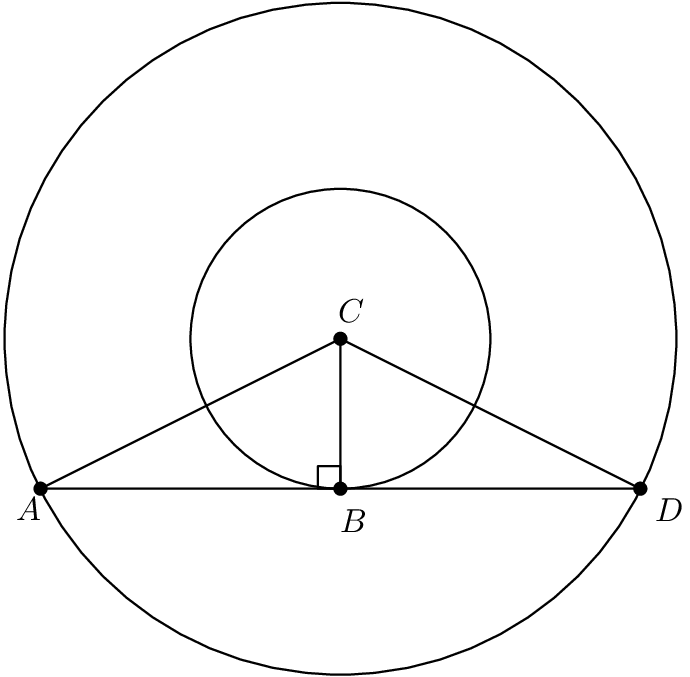
\includegraphics[height=0.4\textheight]{circle5.png}
    \end{figure}
\end{frame}
\begin{frame}{Circle-5}
    \begin{ques}[AMC 8, 2010-23]
        求两个半圆面积之和与大圆面积之比.
    \end{ques}
    \begin{figure}
        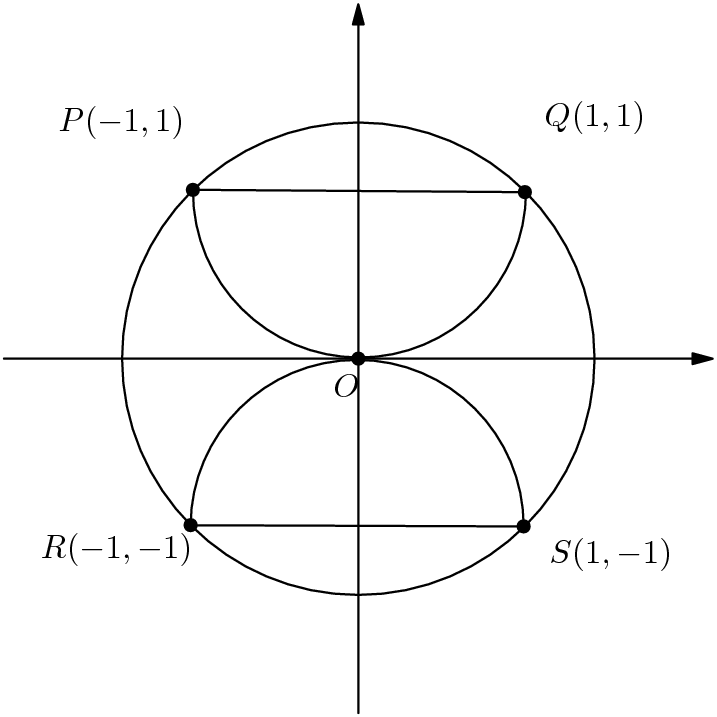
\includegraphics[height=0.4\textheight]{circle6.png}
    \end{figure}
\end{frame}



\begin{frame}{更多资源}
    想探索更多数学或者数学竞赛相关知识, 有如下书目可以参考:
    \cite{潘承洞2003初等数论},\cite{美国数学竞赛指南},\cite{组合数学}.
    \bibliography{geometry2}
    \bibliographystyle{plain}%终端输入bibtex+文件名再ctrl+s两次,plain(数字起头) alpha(字母起头),cd 进入下一级别 cd..返回上一级
\end{frame}
\begin{frame}
    获取数学相关工具和网站:
    \begin{itemize}
        \item MathStackExchange(\url{https://math.stackexchange.com})
        \item AoPS(\url{https://artofproblemsolving.com/wiki/index.php})
        \item Geogebra(\url{https://www.geogebra.org/download})
    \end{itemize}
    数学内容排版软件: Latex(课件均由Latex制作)

    数学相关编程工具: C++,Python, Matlab.
\end{frame}

\end{document}